
In this section we will work through an example of creating and
testing a pattern in the framework.  Our example will be a gossip-like
protocol.  Gossiping is a class of protocols where a particular network
state is updated in the network using periodic/random continuous
messaging.  Gossip-like protocols can be implemented using either
broadcast mechanisms or unicast mechanisms.  In this
example we will implement a unicast-based Gossip (which is
closer to Tuscarora's design philosophy). The state being kept
up to date is simply an integer number that increases monotonically.
The nodes in the network ``gossip'' with each other to make sure they
have the highest/latest number. The code for this example can be
found in the release in the directories
\FilePath{TuscaroraFW/Src/Pattern/Gossip} and \FilePath{TuscaroraFW/Tests/Patterns/Gossip}.


Let's define some basic primitives for the Gossip pattern; 
then we show how to implement these primitives. 


\begin{enumerate}
\item  The pattern sends a status message to selected neighbors at
  random intervals, with some average period---say, 200ms. It uses a
  uniform random number generator and the events module to achieve
  this.  

\item New discovered neighbors are selected to be notified with the
  next status message.

\item If the status info of a received message is older than the
  stored information, its sender is selected to be notified with the
  next status message.

\item  If no new neighbors were selected to be notified, one neighbor
  is selected randomly from the set of neighbors.

\item The list of selected neighbors is cleared after sending a status
  update.

\item If the packet send to a neighbor fails, that neighbor is
  selected again to be notified with the next status message.
\end{enumerate}

\section{Pattern Overview and Definition} \label{sec:PatternCreation}
%\subsection{Pattern Overview}
Operation of the framework and the patterns are asynchronous.
Pattern issues \TuscConcept{Commands} to the Framework, through the PatternBase \CPPVarName{FRAMEWORK} variable. 
For the responses of these \TuscConcept{Commands} as well as 
changes in the pattern neighborhood, 
changes in the status of the previously send packets, and
incoming packets to the pattern,
the framework generates \TuscConcept{Events} and sends them back to the Patterns. 

It is advised that Patterns derive from \CPPClassName{PatternBase} class, since it helps automating registration and bootstrapping procedures of patterns. However, a pattern writer could choose to implement his Pattern from scratch.
\CPPClassName{PatternBase} also provides standard methods that help registering the pattern with the framework. 
In addition to that, it defines virtual functions, one corresponding to each type of \TuscConcept{Event} generated by the Framework, namely 
\begin{itemize}
 \item \CPPFuncName{ReceiveMessageEvent} for handling message receptions, 
 \item \CPPFuncName{NeighborUpdateEvent} for neighbor notifications, 
 \item \CPPFuncName{DataStatusEvent} for handling data notifications, and 
 \item \CPPFuncName{ControlResponseEvent} for handling control responses
\end{itemize}
These functions should be implemented by patterns derived from the \CPPClassName{PatternBase} class.

The code below shows a simple implementation for our \CPPClassName{Gossip} pattern.  


\begin{lstlisting}[style=boralargefile][label={List:Gossip.h}]
/*
 * Gossip.h
 *
 *  Created on:  March 3, 2015
 *     Authors: Mukundan Sridharan, Bora Karaoglu
 */

#ifndef GOSSIP_H_
#define GOSSIP_H_

#include <Types/BasicTypes.h>
#include <Interfaces/Pattern/PatternBase.h>
#include <Lib/Math/Rand.h>
#include "Lib/PAL/PAL_Lib.h"//include the PAL layer
#include "Lib/DS/AVLBinarySearchTreeT.h"

using namespace PWI;

namespace Patterns {

typedef AVLBSTElement<NodeId_t> GossipNeigborContainerTypeElement;
typedef AVLBST_T<NodeId_t> GossipNeigborContainerType;

class GossipLinkComparator: public LinkComparatorI {
public:
  //GossipLinkComparator();
  bool BetterThan (Core::LinkMetrics& A, Core::LinkMetrics& B){
   return (A.quality > B.quality);
  }
};

class Gossip : public PatternBase{
  uint32_t currentStatusId; //Status of the gossip protocol
  FrameworkAttributes fwAttributes;
  uint32_t nonce;
  //Pattern Specific
  UniformRandomInt *rand; //A random number generator
  Event *randEvent_SendUpdate;	//A pointer for the event class used to send random updates
  Event *randEvent_UpdateVar;	//A pointer for the event class used to update stored information
  EventDelegate *eventDel_SendUpdate;//delegate for the random data send event.
  EventDelegate *eventDel_UpdateVar;//delegate for the random data send event.

  void RandomSendHandler(EventDelegateParam param); //Handler for the event generator used to send random updates
  void UpdateVariableHandler(EventDelegateParam param);  //Handler for the event generator used to update stored information

  PatternNeighborTableI *myNbrHood;
  //GossipLinkComparator *myLinkComparator;

  GossipNeigborContainerType SelectedNeighborList; //Set of selected neighbors to send a status update

  FMessage_t& PrepareStatusUpdate();	//Broadcast your status
  void SendMessage();      //Sends a message to the list of selected neighbors
  
  bool SelectNeighbors(NodeId_t nbr); //Add a neighbor to the set of selected neighbors
  void AdjustSelectedNeighbors(); //Make sure at least one neighbor is selected
  void ClearSelectedNeighborList(); //Clear the list of selected neighbors

  NodeId_t IterateThroughNeighbors(uint16_t table_index);
  bool InitiateProtocol();
  void Handle_AttributeResponse(ControlResponseParam response);
  void Handle_LinkThresholdResponse(ControlResponseParam response);
  void Handle_SelectDataNofiticationResponse(ControlResponseParam response);
public:
  //Common to most patterns

  Gossip();	//constructor
  bool Start();  //Lets the test code or network admin start the pattern
  bool Stop(); //Lets the test code or network admin stop the pattern
  
  void NeighborUpdateEvent (NeighborUpdateParam nbrUpdate);
  void ControlResponseEvent (ControlResponseParam response);
  void DataNotificationEvent (DataNotifierParam notification);
  void ReceiveMessageEvent (FMessage_t& msg);
};

} //end of namespace

#endif //GOSSIP_H_
\end{lstlisting}
\label{List:Gossip.h}

The code below shows the definitions provided by the  \CPPClassName{PatternBase} class.  

\begin{lstlisting}[style=boralargefile][label=List:PatternBase.h]
/*
 * PatternI.h
 *
 * 	Author: Mukundan Sridharan
 * 	This is an abstract base class for patterns to derive and implement, to make it easy for registrating with framework and to start them.
 */

#ifndef PATTERN_BASE_H_
#define PATTERN_BASE_H_

#include <Types/BasicTypes.h>
#include <Types/FrameworkTypes.h>
#include <PAL/Delegate.h>
#include <Interfaces/PWI/Framework_I.h>
#include <Interfaces/Core/PatternNamingI.h>


using namespace PAL;
using namespace PWI;
using namespace PWI::Neighborhood;

namespace Patterns {
  //A enum to keep track of Pattern Framework interaction state;
  enum PatternStateE {
    NO_PID,
    GOT_PID,
    REGISTERED,
    EXECUTING,
    ERROR,
  };
  
  enum PatternRequestStateE {
    NONE_PENDING,
    WAITING_FOR_CONTROL_RESPONSE,
    WAITING_FOR_DATA_RESPONSE
  };
///Defines the abstract base class for patterns
class PatternBase {
protected:
  /*
   * @brief Returns a reference to the Pattern's custom neighbor table
   * 
   * @param patternId Pattern's instance ID.
   * @return PWI::Neighborhood::PatternNeighborTableI&. Reference to the patterns neighborhood table.
  
  virtual PatternNeighborTableI& GetNeighborTable(PatternId_t patternId)  = 0;
  */
  
  
protected:
  PatternId_t PID;
  Framework_I* FRAMEWORK;
  bool registered;
  PatternRequestStateE requestState;
  PatternStateE patternState;
  
  virtual void ReceiveMessageEvent (FMessage_t &msg)=0;
  virtual void NeighborUpdateEvent (NeighborUpdateParam nbrUpdate) =0;
  virtual void DataNotificationEvent (DataNotifierParam notification) =0;
  virtual void ControlResponseEvent (ControlResponseParam response) = 0;
  
  void RegisterPattern(PatternId_t pid, PatternTypeE _type);
  void Handle_PatternIDResponse(ControlResponseParam response);
  void Handle_RegisterResponse(ControlResponseParam response);

  
public:
  RecvMessageDelegate_t *recvDelegate;
  NeighborDelegate *nbrDelegate;
  DataflowDelegate_t *dataflowDelegate;
  ControlResponseDelegate_t *controlDelegate;
  /////////////////// Registration and Instantiation Service ////////////////////
  //PatternBase(PatternTypeE type); 
  PatternBase(PatternTypeE type, char uniqueName[128]);
  ///Starts the pattern, must be implemented by each pattern.
  virtual bool Start()=0;
  virtual bool Stop()=0;

  ///Virtual destructor
  virtual ~PatternBase(){}
};

}//End of namespace

#endif /* PATTERN_BASE_H_ */
\end{lstlisting}

\section{Pattern Flow}

Before going into the implementation details, lets look at the flowchart in \cref{fig:PatternFlowChart} that show how the pattern is initialized and is integrated with the framework. \Cref{fig:PatternFlowChart} is divided into 3 sections corresponding the state of the pattern; \CPPConstant{UNREGISTERED}, \CPPConstant{REGISTERED}, and \CPPConstant{EXECUTING}.

%The framework supports usage of both external and internal naming services for obtaining pattern IDs (PID). 
%Patterns using framework supported naming service get their IDs from the framework with the registration response. 
%Hence, for patterns using internal naming services
%\CPPConstant{UNREGISTERED}, and \CPPConstant{GOT\_PID} states are combined and the pattern state changes from \CPPConstant{NO\_PID} to \CPPConstant{REGISTERED} with the reception of a positive registration response. 
%The \CPPClassName{Gossip}, too, employs framework supported naming service and gets its PID with a registration response.  

\begin{figure}[t]
 \centering
 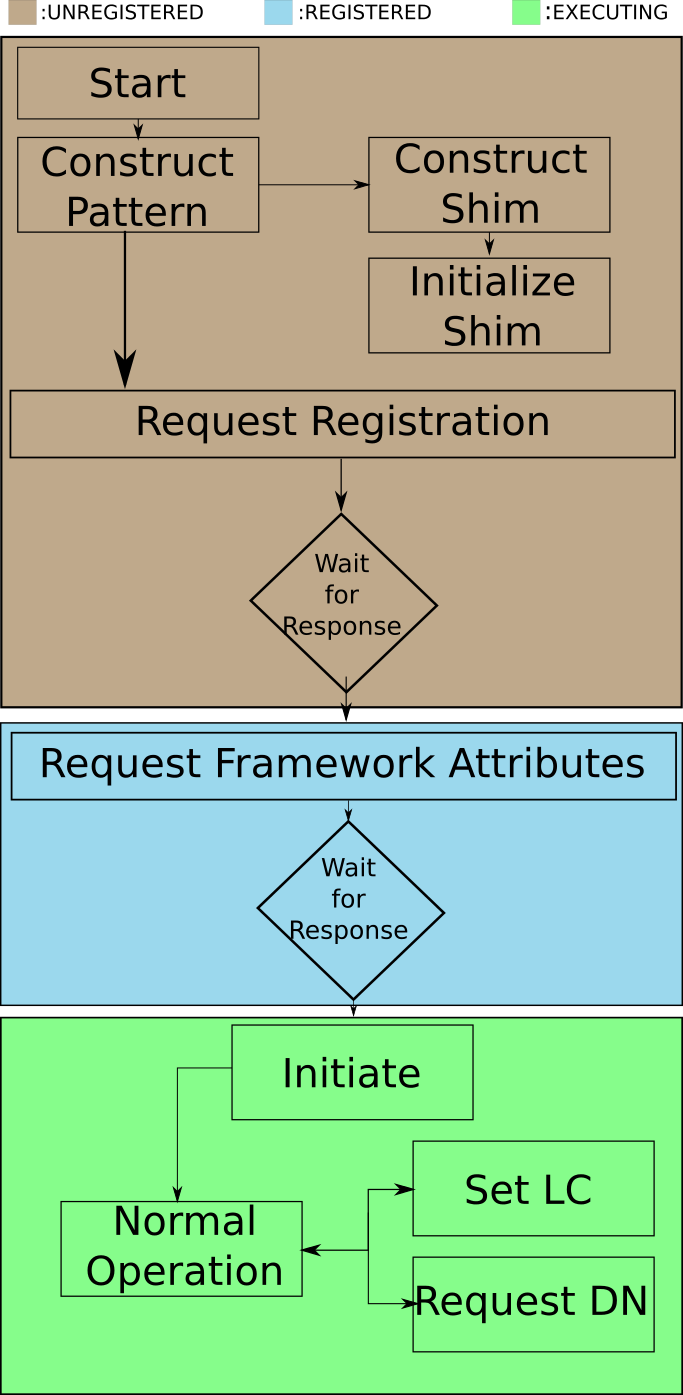
\includegraphics[width=0.4\linewidth]{figures/PatternFlowChart}
 \caption{Flow chart of pattern initialization and registration}
 \label{fig:PatternFlowChart}
\end{figure}



First, the pattern object is constructed. This constructor initializes various parameters of a pattern. 
Next, a shim layer implementing platform specific functions is created. 
Our simple pattern is deriving from \CPPClassName{PatternBase} and call \CPPClassName{PatternBase}'s constructor explicitly that
constructs and initializes the shim layer. 



Initialization of the shim layer 
initializates the internal variables and stores the delegates used for callbacks back to the pattern, namely
\CPPFuncName{ReceiveMessageEvent}, \CPPFuncName{NeighborUpdateEvent},
\CPPFuncName{DataNotificationEvent}, and
\CPPFuncName{ControlResponseEvent}.
However, it does not automatically initiate the registration of the pattern with the framework. \TuscConcept{Patterns} explicitly request registration with the framework and handle framework's response through \CPPFuncName{ControlResponseEvent} function. 

Gossip's PID is assigned by the framework. This PID is included in the positive response to the pattern's registration request,
Receiving a positive response to the pattern's registration request, pattern changes state from \CPPConstant{UNREGISTERED} to \CPPConstant{REGISTERED}. 
At this stage, framework is queried for its attributes. 

By receiving the response to framework attributes request, pattern's state changes to \CPPConstant{EXECUTING}. 
In this state, the pattern initiates its operation and starts operating normally. 
In the beginning of its operation, a pattern can set its link comparator and subscribe to the data notifications of interest. 
However, these operations can be repeated anytime during the normal operation to change the link comparator or to change pattern's subscription to data notifications.  

In the following sections, we will investigate how \CPPClassName{Gossip} implements various functions for its operations.  



\section {Initialization} \label{sec:Initialization}
Patterns deriving from \CPPClassName{PatternBase} initialize their shim layer through \CPPClassName{PatternBase}'s constructor. 
%, which requires a pattern type and a unique string differentiating different instances of the same pattern. 
%\CPPClassName{Gossip}'s constructor further initializes \CPPClassName{Gossip}'s neighborhood by passing criteria for minimum acceptable limits for a link to be accepted in pattern's neighborhood,
%and a comparator for sorting the links to the framework. Next,
%\CPPClassName{Gossip} notifies the framework about the type of
%acknowledgements that it is interested in, namely destination-oriented
%acknowledgments such as a successful (or unsuccessful) reception of
%the packet (indicated by \emph{PDN\_RECV\_DEST\_MASK}), and the acknowledgement
%indicating the availability of the framework to receive packets
%(indicated by \emph{PDN\_WF\_SENT\_MASK}). Finally, \CPPClassName{Gossip} initializes a
%random number generator, two event delegates that are used to schedule
%future events, and the status information to be gossiped.  
\CPPClassName{Gossip}'s constructor further initializes 
\begin{itemize}
	\item two event delegates that are used to schedule
	future events, 
	\item a timer delegate that is used to resend messages in case a message gets lost before getting received by the framework
	\item a random number generator,
	\item a table that stores neighbors,
	\item a nonce and a boolean variables facilitating message passing between the pattern and the framework, and 
	\item internal gossip variables for keeping the status of the gossiped information,
\end{itemize}


\begin{lstlisting}[style=boralargefile][label=List:Gossip.cc:Constructor]
Gossip::Gossip() : PatternBase(Core::Naming::GOSSIP_PTN, (char*)"Gossip_1"){
	Debug_Printf(DBG_PATTERN, "Gossip::Initializing\n");


	//delegate handles to the events
	eventDel_SendUpdate = new EventDelegate(this, &Gossip::RandomSendHandler);
	eventDel_UpdateVar = new EventDelegate(this, &Gossip::UpdateVariableHandler);
	eventDel_ReSendUpdate = new TimerDelegate(this, &Gossip::ReSendHandler);


	//Creates a uniform random number with mean 200,000 and with range +/_100,000
	//That is the values vary between 100,000 to 300,000
	UniformRNGState _state;
	_state.cmrgState.stream = MY_NODE_ID;
	_state.mean = MeanUpdateInterval;
	_state.range = RangeUpdateInterval;
	rand = new UniformRandomInt(_state);

	//Initialize pattern neighbor table
	myNbrHood = new PatternNeighborTable(QUALITY_LC);

	//Initialize variables facilitating message passing
	nonce=1;
	hasFWRejectedPacket = false;

	//Initialize Gossip status
	currentStatusId = 0;
}
\end{lstlisting}

\section {Starting} \label{sec:Starting}

\CPPClassName{Gossip} starts registering itself with the framework with its \CPPFuncName{Start} method. 
In this method, \CPPClassName{Gossip}
initiates pattern registration. 

The framework supports usage of both external and internal naming services for obtaining unique pattern IDs (PID). 
Patterns using framework supported naming service get their IDs from the framework with the registration response while if there is an external service, Pattens can get a PID using this external service prior to registration and include the obtained PID in their registration request. 

Gossip does not have an external pattern naming service and its pattern ID (PID) assigned by the framework during registration. In its registration request, Gossip uses a null \CPPVarName{PID} of 0 together with a unique string identifier of the pattern. The string identifier is used by the framework in generating a \CPPVarName{PID}. 

\begin{lstlisting}[style=boralargefile][label=List:Gossip.cc:Start]
bool Gossip::Start(){
	Debug_Printf(DBG_PATTERN, "Gossip::Start Starting gossiping \n");
	Debug_Printf(DBG_PATTERN, "Gossip:: Sending the RegisterPattern Request to framework...\n");

	FRAMEWORK->RegisterPatternRequest (PID, uniqueName, Core::Naming::GOSSIP_PTN);
	++n_ExpectedFrameworkResponses;
	return true;
}
\end{lstlisting}


\section {Control Response Event Handling} \label{sec:ControlResponseEvent}

The Events related to the control plane are handled by the  \CPPFuncName{ControlResponseEvent} function, which is declared as virtual by the \CPPClassName{PatternBase} class and must be implemented by all patterns deriving from it. 

\CPPClassName{PatternBase} has two internal variables, \CPPVarName{n\_ExpectedFrameworkResponses} and \CPPVarName{patternState}, which help keeping the state of the messaging interface between the patterns and the framework.  

\CPPVarName{patternState} can take values of 
\CPPConstant{NO\_PID},
\CPPConstant{GOT\_PID},
\CPPConstant{REGISTERED}, and
\CPPConstant{EXECUTING}. 
It is updated by a pattern at each stage of the registration process.

%\bk{Again we have to recheck this. how is it moved from \CPPConstant{REGISTERED} to \CPPConstant{EXECUTING} is not clear since it depends on multiple responses. Again, we can use a count instead of absolute state.   }

Patterns expect different responses from the framework depending on their association status. 
%In the case of an unexpected response, \CPPFuncName{ControlResponseEvent} function generates a debug statement. Otherwise, it directs the responses from the framework to the handler functions.
In general, the 
\CPPFuncName{ControlResponseEvent} function implementation should filter out unexpected responses%
\footnote{
An example situation in which an unexpected response might be received from the framework occurs when a pattern crashes and restarts without the crash being detected by the Framework.  
In this case, framework can potentially continue sending responses to earlier requests by the crashed pattern instance.}
and implement error handling for unexpected events from Framework. 

%\bk{We should maybe make the handling of Handle\_RegisterResponse seemsless to the pattern. One method of achieving this could be handling responses with a different funtion at the PatternBase by default and directing it to the Pattern for any response other than PWI::PTN\_RegisterResponse type. }

\begin{itemize}
\item In \CPPConstant{NO\_PID} state, \CPPClassName{Gossip} 
%has just passed its registration request and 
is only expecting a registration response. 
Registration is completed by calling  \CPPClassName{PatternBase}'s \CPPFuncName{Handle\_RegisterResponse}. Next, \CPPClassName{Gossip} queries for the attributes of the framework. 

\item In \CPPConstant{REGISTERED} state, \CPPClassName{Gossip} expects a response to its query for the attributes of the framework. The response for this query is handled in \CPPFuncName{Handle\_AttributeResponse}, which stores the framework attributes and updates \CPPVarName{patternState}.

\item In \CPPConstant{EXECUTING} state, the registration is completed and the pattern is operational. 
In this state the pattern receives responses to various directives that it passes to the framework. 
%Although, there are 6 possible responses in this state, only 
%\CPPConstant{PTN\_SelectDataNotificationResponse}, 
%\\ \CPPConstant{PTN\_SetLinkThresholdResponse}, and 
%\CPPConstant{PTN\_AttributeResponse} 
%are relevant for \CPPClassName{Gossip}. 

	\begin{itemize}
	\item \CPPConstant{PTN\_SelectDataNotificationResponse}: 
	Framework responds to the pattern's selection of data notifications with this response. 
	\CPPClassName{Gossip} handles this response with  \\ \CPPFuncName{Handle\_SelectDataNofiticationResponse}, which checks the success or the failure of the request and generate debug messages. 
	%in addition to updating \CPPVarName{requestState} and \CPPVarName{patternState} variables.
	%\bk{We should handle the case of negative status gracefully. Maybe Start function could be rescheduled attempting to restatr registration procedure.}
	In the case of a failure, \CPPFuncName{The SelectDataNotificationsRequest()} function is called to issue a new request to the framework to set the appropriate data notification masks.
	
	\item \CPPConstant{PTN\_SetLinkThresholdResponse}: 
	Framework responds to the pattern's selection of link threshold with this response. 
	\CPPClassName{Gossip} handles this response with \\ \CPPFuncName{Handle\_LinkThresholdResponse}, which checks the success or the failure of the request and generate debug messages. 
	%in addition to updating \CPPVarName{requestState} and \CPPVarName{patternState} variables.
	%\bk{We should handle the case of negative status gracefully. Maybe a different threshold response is scheduled.}
	In the case of a failure, \CPPFuncName{SetNeighborhoodandLinkComparator()} function is recalled issuing a new request to the framework for link comparator and threshold. 
	
	\item \CPPConstant{PTN\_AttributeResponse}: 
	This is a notification indicates some change in framework's attributes. \CPPClassName{Gossip} handles this response with \CPPFuncName{Handle\_AttributeResponse} function similar to the \CPPConstant{REGISTERED} state.
	
	\item \CPPConstant{PTN\_AddDestinationResponse}: 
	This is the framework's response to a request to add a destination(s) to the list of destinations of a previous packet before it is sent out of the waveform.   
	Not used by \CPPClassName{Gossip}.
	
	\item \CPPConstant{PTN\_ReplacePayloadResponse}: 
	This is the framework's response to a request to replace the payload of a previous packet before it is sent out of the waveform.   
	Not used by \CPPClassName{Gossip}.
	
	\item \CPPConstant{PTN\_CancelDataResponse}: 
	This is the framework's response to a request to stop one of its previous packets before it is sent out of the waveform.  
	Not used by \CPPClassName{Gossip}.
	
	
	\end{itemize}

\end{itemize}


\begin{lstlisting}[style=boralargefile] [label=List:Gossip.cc:ControlResponseEvent]
void Gossip::ControlResponseEvent(ControlResponseParam response)
{
	Debug_Printf(DBG_PATTERN, "Gossip:: Got a control response of type %d\n", response.type);
	switch (patternState){
	case NO_PID:
	case GOT_PID:
		if(response.type == PWI::PTN_RegisterResponse){
    		--n_ExpectedFrameworkResponses;
			Handle_RegisterResponse(response);
			FRAMEWORK->FrameworkAttributesRequest(PID);
			++n_ExpectedFrameworkResponses;
		}else {
			Debug_Printf(DBG_PATTERN, "Gossip:: ControlResponseEvent: My state is %d I got wrong response type %d\n", patternState, response.type);
		}
		break;
	case REGISTERED:
		if(response.type == PWI::PTN_AttributeResponse){
    		--n_ExpectedFrameworkResponses;
    		Handle_AttributeResponse(response);
    		InitiateProtocol();

		}else {
			Debug_Printf(DBG_PATTERN, "Gossip:: ControlResponseEvent: My state is %d, I got wrong response type %d\n", patternState,response.type);
		}
		break;
	case EXECUTING:
		switch(response.type){
		case PTN_SelectDataNotificationResponse:
            Handle_SelectDataNofiticationResponse(response);
            --n_ExpectedFrameworkResponses;
			break;
		case PTN_SetLinkThresholdResponse:
			Handle_LinkThresholdResponse(response);
			--n_ExpectedFrameworkResponses;
			break;
		case PTN_AttributeResponse:
    		--n_ExpectedFrameworkResponses;
    		Handle_AttributeResponse(response);
    		InitiateProtocol();
    		break;
		case PTN_AddDestinationResponse:
		case PTN_ReplacePayloadResponse:
		case PTN_CancelDataResponse:
		default:
			Debug_Printf(DBG_PATTERN, "Gossip:: ControlResponseEvent: My state is %d, I got wrong response type %d\n", patternState,response.type);
			break;
		}
		break;
		default:
			break;
	}
}


void Gossip::Handle_AttributeResponse(ControlResponseParam response){
	FrameworkAttributes *atr = (FrameworkAttributes*) response.data;
	fwAttributes = *atr;

	if( patternState == REGISTERED) {
		patternState = EXECUTING;
	}
	else {
		 Debug_Printf(DBG_PATTERN, "PatternBase::Pattern getting initiated without registration.\n");
	}

	Debug_Printf(DBG_PATTERN,"Gossip:: Handle_AttributeResponse: Framework supports %d waveforms, with max pkt size is %d .\n", fwAttributes.numberOfWaveforms, fwAttributes.maxFrameworkPacketSize);
	for(uint i=0; i<fwAttributes.numberOfWaveforms; i++){
		Debug_Printf(DBG_PATTERN, "Gossip::Handle_AttributeResponse: Waveform %d Id is %d\n", i, fwAttributes.waveformIds[i]);
	}
}
\end{lstlisting}

\section {Initiation} \label{sec:Initiation}

With the reception of a positive response to its registration request, \CPPClassName{Gossip} initiates its operation with \CPPFuncName{InitiateProtocol()} function.

In this function, \CPPClassName{Gossip} calls \CPPFuncName{SetNeighborhoodandLinkComparator()} to select
%Patterns select 
(i) a link comparator type defining the criteria for differentiating between links, and 
(ii) a threshold defining minimum acceptable limits for a link to be accepted in pattern's neighborhood. 
%Both the comparator and the threshold are passed to the framework. 
\CPPClassName{Gossip} selects the link quality as the criterion to differentiate between links and sets its threshold to a quality level of 0.1. 

Next, by calling \CPPFuncName{RequestDataNotifications()} function,
\CPPClassName{Gossip} notifies the framework about the type of acknowledgements that it is interested in, 
namely destination-oriented acknowledgments 
such as a successful (or unsuccessful) reception of the packet (indicated by \CPPConstant{PDN\_RECV\_DEST\_MASK}).
%and the acknowledgement indicating the availability of the framework to receive packets (indicated by \CPPConstant{PDN\_WF\_SENT\_MASK}).


%These settings finalize \CPPClassName{Gossip}'s configuration and 
Finally, \CPPClassName{Gossip} initiates its operation by starting two random event generators used for (i) periodically sending messages and updating the
information (see the next section). 
These random event generators are stopped in \CPPClassName{Gossip}'s stop routine, which stops the operation of the pattern. 

%Finally, a timer, \CPPVarName{randEvent\_ReSendUpdate}, is initialized. This timer is rescheduled when a data message is sent and is used for resending message to the framework if a response is not received for a \CPPVarName{ReSendTimeOutInterval}.  

\begin{lstlisting}[style=boralargefile][label=List:Gossip.cc:InitiateProtocol]
bool Gossip::InitiateProtocol(){
	//Initialize neighborhood and set link comparator.
	SetNeighborhoodandLinkComparator();

	//tell framework which notifications you are interested in
	RequestDataNotifications();

	Debug_Printf(DBG_PATTERN, "Gossip::Have configured everything succeessfully. Good to go. \n");

	uint64_t eventDelay = rand->GetNext();
	//The event callback will have null parameter
	randEvent_SendUpdate = new Event(eventDelay, *eventDel_SendUpdate, (void *) 0);
	randEvent_UpdateVar = new Event(eventDelay, *eventDel_UpdateVar, (void *) 0);

	randEvent_ReSendUpdate = new Timer(ReSendTimeOutInterval, ONE_SHOT, *eventDel_ReSendUpdate);
	randEvent_ReSendUpdate->Suspend();
	return true;
}

void Gossip::SetNeighborhoodandLinkComparator(){
	FRAMEWORK->SelectLinkComparatorRequest(PID,PWI::Neighborhood::QUALITY_LC);
	++n_ExpectedFrameworkResponses;
	//FRAMEWORK->SelectLinkComparatorRequest (PID, QUALITY_LC);
	LinkMetrics myThreshold;
	myThreshold.quality = 0.10;


	FRAMEWORK->SetLinkThresholdRequest(PID,myThreshold);
	requestState = WAITING_FOR_CONTROL_RESPONSE;
	++n_ExpectedFrameworkResponses;
}

void Gossip::RequestDataNotifications(){
	uint8_t mask = PDN_RECV_DEST_MASK;
	FRAMEWORK->SelectDataNotificationRequest(PID, mask);
	requestState = WAITING_FOR_CONTROL_RESPONSE;
	++n_ExpectedFrameworkResponses;
}
\end{lstlisting}


\section {Data Status Handling} \label{sec:DataNotificationEvent}

Packet related notifications are handled with \CPPFuncName{DataStatusEvent(DataStatusParam ntfy)}. 
The patterns notify the framework about the type of notifications that they are interested in. They can change this request anytime throughout the course of operation. For a full list of notifications please refer to the TuscaroraFramework\_API documentation.

In its start routine, \CPPClassName{Gossip} passes its interest on two types of acknowledgements: 
\begin{itemize}
\item \CPPConstant{PDN\_RECV\_DEST\_MASK}: Since \CPPClassName{Gossip} registers for this type, it will be notified about
whether a packet was successfully received via a \CPPClassName{DataNotifierParam} with a \CPPVarName{ackType} of \CPPConstant{PDN\_DST\_RECV}. 
%Each notification includes information about \CPPVarName{ntfy.noOfDest} listed in the array \CPPVarName{ntfy.dest[]}. 
\CPPVarName{ntfy.status} indicates the success or the failure of the reception by the \CPPVarName{ntfy.noOfDest} destinations listed in the array, \CPPVarName{ntfy.dest[]}.
For negative acknowledgements, \CPPClassName{Gossip} adds the list of negatively acknowledged destinations into its list of neighbors to be updated in the next cycle. 

%\bk{The source code is modified to include the suggested changes. It should be rechecked before the release }

\item \CPPConstant{PDN\_FW\_RECV\_MASK}: This notification type is on by default for all patterns and is generated without requiring to ask for it. Framework notifies \CPPClassName{Gossip} whether it accepts the previous packet sent by the pattern via a \CPPClassName{DataNotifierParam} with a \CPPVarName{ackType} of \CPPConstant{PDN\_FW\_RECV}. \CPPVarName{ntfy.status} indicates whether the packet is accepted or rejected. 
With the reception of the response, \CPPClassName{Gossip} 
cancels the timer that resends packets after a timeout period after which no response is received. 
For accepted packets, \CPPClassName{Gossip} further clears the list of selected neighbors, and increments \CPPVarName{nonce} variable used to identify packets not yet assigned a packet id.
For rejected packets, \CPPClassName{Gossip} further checks \CPPVarName{ntfy.readyToReceive} parameter that indicate whether the framework is accepting new packets at that moment and resends a status update with the same \CPPVarName{nonce} id if it does. 
On the other hand, if the framework indicates that it is not ready to accept packets, \CPPClassName{Gossip} sets the \CPPVarName{hasFWRejectedPacket} variable preserving the state. 
In that state, \CPPClassName{Gossip} tries sending a new status update%
\footnote{but with the same nonce id since it is not matched to any messages yet}
with the reception of a future data notification (of any \CPPVarName{ackType}) that indicates the availability of the framework to receive packets.   

\end{itemize}

\begin{lstlisting}[style=boralargefile] [label=List:Gossip.cc:ReceiveDataNotifications]
void Gossip::ReceiveDataNotifications(DataNotifierParam ntfy) {
	///You have received ack for previous message.
	//check what happened to the previous message
	Debug_Printf(DBG_PATTERN,"Gossip:: Received a data notification from framework\n");
	switch (ntfy.type){
		case ACK_DST_RECV:
			if(!ntfy.status ){
				Debug_Printf(DBG_PATTERN,"Gossip:: Message id %d not received by destination\n", ntfy.messageId);
				SelectNeighbors(ntfy.dest);
			}
		break;
		case READY_TO_RECV:
			SendMessage();
		break;
		default:
		break;
	}
}
\end{lstlisting}

\section {Neighbor Updates} \label{sec:NeighborUpdateEvent}
Neighbor related notifications are handled by
\CPPFuncName{NeighborUpdateEvent(NeighborUpdateParam nbrUpdate)}, which
is defined as virtual by the \CPPClassName{PatternBase} and must be implemented by all patterns deriving from it. 
%In the registration process with the framework, \CPPClassName{PatternBase} class defines this function as the target for the neighbor update events. 

For each change in the pattern neighborhood, the framework notifies the pattern with a \CPPVarName{NeighborUpdateParam} that has a \CPPVarName{changeType} of  
\begin{itemize}
\item \CPPVarName{NBR\_NEW} for detected links, 
\item \CPPVarName{NBR\_DEAD} for links that are detected as broken or not satisfying the threshold conditions specified,
\item \CPPVarName{NBR\_UPDATE} for links that remain in neighborhood but change some properties.
\end{itemize}
%(i)~links that are discovered and links that are detected with an \CPPVarName{nbrUpdate.changeType} of \emph{NBR\_NEW}, 
%(ii)~links that aredetected as broken or not satisfying the threshold conditions specified with an \emph{nbrUpdate.changeType} of \emph{NBR\_DEAD},
%(iii)~links that remain in neighborhood but change some propertieswith an \emph{nbrUpdate.changeType} of \emph{NBR\_UPDATE}.  
\CPPClassName{Gossip} uses the \CPPFuncName{UpdateTable(NeighborUpdateParam \_param)} of the \CPPClassName{PatternNeighborTable} to make the corresponding changes in the \CPPVarName{myNbrHood}.

\begin{lstlisting}[style=boralargefile][label=List:Gossip.cc:NeighborUpdateEvent]
void Gossip::NeighborUpdateEvent(NeighborUpdateParam nbrUpdate)
{
  myNbrHood->UpdateTable(nbrUpdate);
}
void Patterns::PatternNeighborTable::UpdateTable(NeighborUpdateParam _param)
{
	//bool signalPattern=false;
	LinkMap *newLink;Link *ptnLink;
	switch(_param.changeType)
	{
	case NBR_NEW:
		newLink = new LinkMap(_param.link.linkId, _param.link);
		nbrhood->Insert(newLink);
		//signalPattern =true;
		break;
	case NBR_DEAD:
		if(nbrhood->DeleteLink(_param.link.linkId)){
			//signalPattern =true;
		}
		break;
	case NBR_UPDATE:
		Debug_Printf(DBG_PATTERN, "PatternNeighborTable:: updating neighbor %d on waveform %d\n", _param.nodeId, _param.link.linkId.waveformId);fflush (stdout);
		ptnLink = nbrhood->GetLink(_param.link.linkId);
		if(ptnLink){
			if(ptnLink->linkId.waveformId){
				ptnLink->metrics = _param.link.metrics;
			}
		}else {
			printf("Mismatch in neighbor table status, I (Pattern %d) dont have link (%d, %d) in table, but received an update event \n Created new link\n",
					this->patternId,_param.nodeId, _param.link.linkId.waveformId);
			newLink = new LinkMap(_param.link.linkId, _param.link);
			nbrhood->Insert(newLink);
		}

		break;
	default:
		printf("PatternNeighborTable:: Error: wrong neighbor update signal\n");
		break;
	}
}
\end{lstlisting}

\section {Receiving Messages} \label{sec:ReceiveMessageEvent}

Received messages are handled by \CPPFuncName{ReceiveMessage(FMessage\_t\& msg)}. 
In this function, \CPPClassName{Gossip} compares the status ID reported in the packet with the internal state ID. If the internal state variable (\CPPVarName{currentStatusId})
\begin{itemize} 
\item  is smaller than the one reported in the packet, the internal state variable is updated. 
\item is larger than the one reported in the packet, the source node of the the packet is added to the list of nodes that will be reported in the following period.  
\item is equal to the one reported in the packet, the packet is ignored. 
\end{itemize}  
% XXXXXXXXX KC sez:  I think the ">=" in the following should be "<".
% According to the problem statement above, our state should be the
% highest/latest ID.
% BK: You are right. We should update if the message's status is larger/newer than the internal one.
\begin{lstlisting}[style=boralargefile] [label=List:Gossip.cc:ReceiveMessageEvent]
void Gossip::ReceiveMessageEvent(FMessage_t& msg)
{
  GossipMsg* gMsg = (GossipMsg*) msg.GetPayload();
 Debug_Printf(DBG_PATTERN, "Gossip:: Received msg from %u with status seq %u \n",msg.GetSource(), gMsg->currentStatusId);
  //Process the recevied message
  if(currentStatusId < gMsg->currentStatusId) {
	  currentStatusId = gMsg->currentStatusId;
  }
  else if(currentStatusId > gMsg->currentStatusId) {
	  SelectNeighbors(msg.GetSource());
  }
}
\end{lstlisting}

\section {Handling Scheduled Events} \label{sec:ScheduledEvents}

Next, we implement the handler methods of scheduled events. 
In \CPPClassName{Gossip}, we have two such methods: a method that periodically
sends messages, \CPPFuncName{RandomSendHandler(EventDelegateParam param)}; 
and a method that increments the state of the pattern,
\emph{UpdateVariableHandler(EventDelegateParam param)}. 
Both of these methods are scheduled randomly and reschedule their triggering events when executed. 
When sending an update, if no nodes were selected before, we randomly
select a node using \emph{AdjustSelectedNeighbors()}. 
We make sure
that the selected node is a neighbor and was not already selected
using \emph{SelectNeighbors(NodeId\_t nbr)}.

\begin{lstlisting}[style=boralargefile] [label=List:Gossip.cc:RandomSendHandler]
//Handler for the randEvent_UpdateVar event
void Gossip::UpdateVariableHandler(EventDelegateParam param){
	uint64_t eventDelay = rand->GetNext();
	uint64_t curTime = Debug::GetTimeMicro();
	param.eventPtr->ReSchedule(eventDelay*100,(void *) (0));
	Debug_Printf(DBG_PATTERN, "UpdateVariable:: Rescheduled event to fire at %lu\n",curTime+eventDelay);
	++currentStatusId;
}
//Handler for the RandomSend event
void Gossip::RandomSendHandler(EventDelegateParam param){
  //Lets us first reshedule the event
  uint64_t eventDelay = rand->GetNext();
  uint64_t curTime = Debug::GetTimeMicro();
  param.eventPtr->ReSchedule(eventDelay,(void *) (0));
 Debug_Printf(DBG_PATTERN,"Gossip::RandomSend:: Rescheduled event to fire at %lu\n",curTime+eventDelay);fflush(stdout);
  //Now lets broadcast our status
  AdjustSelectedNeighbors();
  if(SelectedNeighborList.Size() > 0) SendMessage(); //If I have at least one destination send this message
}

void Gossip::AdjustSelectedNeighbors() {
	if(SelectedNeighborList.Size() > 0) return; //Already selected neighbors based on other criteria
	uint16_t nbrCount = myNbrHood->GetNumberOfNeighbors();
	Debug_Printf(DBG_PATTERN,"Gossip:: Got %d neighbors  \n", nbrCount);fflush(stdout);
	if (nbrCount == 0) return;//Return if there are no neighbors to choose from
	NodeId_t sNeighbor;
	uint16_t i=0;
	while(SelectedNeighborList.Size() == 0) {
		uint64_t pickrandom = rand->GetNext();
		pickrandom = pickrandom % nbrCount;
		Debug_Printf(DBG_PATTERN,"Gossip:: Got %d neighbors and picking %lu neighbor from tabel  \n", nbrCount, pickrandom);fflush(stdout);
		PatternNeighborIterator it = myNbrHood->Begin();
		for(uint16_t ii=0; ii< nbrCount; ii++) {
			if(pickrandom == 0) {	
				sNeighbor = (it->linkId.nodeId);
			}
			--pickrandom;
			Debug_Printf(DBG_PATTERN,"Gossip:: Intering neighbortable inde %d neighbor is %d \n",ii, it->linkId.nodeId);fflush(stdout);
			it=it.GetNext();
		}
		/*if(pickrandom == 0) {
			sNeighbor = (it->linkId.nodeId);
		}*/
	      
		
		Debug_Printf(DBG_PATTERN,"Gossip:: Selected %d neighbor \n", sNeighbor);fflush(stdout);
		if( SelectNeighbors(sNeighbor) ) {
			Debug_Printf(DBG_PATTERN,"Gossip:: PickRandomNeighbor %d \n", sNeighbor);fflush(stdout);
		}
		i++;
		Debug_Printf(DBG_PATTERN,"Gossip:: in while %d times  \n", i);fflush(stdout);
	}
}

bool Gossip::SelectNeighbors(NodeId_t nbr){
	if( myNbrHood->GetNeighborLink(nbr) && !(SelectedNeighborList.Search(nbr)) ) { //If the node is my neighbor and not selected before
		Debug_Printf(DBG_PATTERN,"Gossip:: SelectNeighbor: Ading neighbor %d neighbors  to SelectedNeighborList \n", nbr);fflush(stdout);
		return SelectedNeighborList.Insert(nbr);
	}
	return false;
}
}
\end{lstlisting}

\section {Sending Messages} \label{sec:SendingMessages}

Sending status update messages is implemented in
\CPPFuncName{SendMessage()}. 
This method creates a packet containing the
current status information of the node using
\CPPFuncName{PrepareStatusUpdate()}, 
and passes the constructed packet to the framework
along with 
\begin{itemize}
\item an array including the set of previously selected destinations in \CPPVarName{SelectedNeighborList},
\item the size of this array,
\item a temporary pattern generated message ID, namely \CPPVarName{nonce} and
\item a boolen variable indicating whether ACKs are requested. 
\end{itemize}

While sending a message to the framework, pattern should provide a temporary ID to the message called a \CPPVarName{nonce}, which is used to identify a packet until a unique Message ID is generated for the message by the Framework and returned to the Pattern. 
When the framework receives the packet, it generates a \CPPVarName{DataNotifierParam} with an \CPPVarName{ackType} of \CPPConstant{PDN\_WF\_RECV}.  
This \CPPVarName{DataNotifierParam} also includes the \CPPVarName{nonce} generated with the pattern along with the \CPPVarName{messageId} that can be used to uniquely identify the message from that point on.

The nonce is also useful for error detection and recovery, if either the Command from pattern to framework gets lost or if the Data Notification Event with the message ID from the framework gets lost. A pattern in general should start a timer when sending a message to the framework and if a Data Notification for the message is not received before the timer expires, it should resend the same message with the same nonce. If the framework receives two consecutive messages with the same nonce, it would recognize it as a duplicate and resend the data notification for that packet. 
 

\CPPFuncName{SendMessage()} function also schedules an event resending a new packet if no framework response is received in \CPPConstant{ReSendTimeOutInterval}. 
Finally, the \CPPVarName{hasFWRejectedPacket} state variable is cleared since the packet has not been rejected at that time instant. 
This state variable can be set via a data notification as discussed in \cref{sec:DataNotificationEvent}.

%If the framework rejects the message, \emph{SendMessage()} terminates and is re-invoked when the framework later notifies the pattern that it is free to accept messages. If the framework accepts the packet, \emph{SelectedNeighborList} is cleared.
\begin{lstlisting}[style=boralargefile] [label=List:Gossip.cc:SendMessage]
// This function broadcast status
FMessage_t& Gossip::PrepareStatusUpdate(){
	Debug_Printf(DBG_PATTERN, "Gossip:: PrepareStatusUpdate\n");
	
	//Construct packet and send
	FMessage_t *sendMsg;
	//Make sure to use new() operator to create packet on heap.
	sendMsg = new FMessage_t(sizeof(struct GossipMsg));
	sendMsg->SetSource(MY_NODE_ID);
	sendMsg->SetInstance(PID);
	
	GossipMsg* gMsg = (GossipMsg*) sendMsg->GetPayload();
	gMsg->currentStatusId=currentStatusId;
	return (*sendMsg);
}
// This function sends a message to the list of selected neighbors
void Gossip::SendMessage() {
	NodeId_t selnodes[SelectedNeighborList.Size()];
	GossipNeigborContainerTypeElement* elptr = SelectedNeighborList.Begin();
	int i=0;
	while(elptr){
		selnodes[i] = elptr->data;
		elptr = SelectedNeighborList.Next(elptr);
		++i;
	}
	Debug_Printf(DBG_PATTERN, "Gossip::SendMessage multicasting to %d destinations \n", SelectedNeighborList.Size()); fflush(stdout);
	MessageId_t msgID = FRAMEWORK->Send(selnodes, (uint16_t) SelectedNeighborList.Size(), PrepareStatusUpdate(), (U64NanoTime*) NULL, false);
	
	if (msgID == 0){
		Debug_Printf(DBG_PATTERN, "Gossip::SendMessage framework is busy. Rejected the packet. Keeping list of neighbors.\n"); fflush(stdout);
	}
	else{
		Debug_Printf(DBG_PATTERN, "Gossip::SendMessage framework accepted message (%d). \n", msgID);fflush(stdout);
		ClearSelectedNeighborList();
	}
}

void Gossip::ClearSelectedNeighborList(){
	GossipNeigborContainerTypeElement *elptr,*elptr2;
	elptr = SelectedNeighborList.Begin();
	while(SelectedNeighborList.Size()>0){
		elptr2 = SelectedNeighborList.Next(elptr);
		SelectedNeighborList.DeleteElement(elptr);
		elptr = elptr2;
	}
}
\end{lstlisting}

\section {Broadcasting a Message } \label{sec:BroadcastingMessages}

While \CPPClassName{Gossip} primarily uses generic \CPPFuncName{SendData} API, sending a broadcast message is quite similar. The primary
difference is that, 
while generic \CPPFuncName{SendData} primitive addresses to one or more destinations, 
a broadcast is addressed to a particular waveform.
The framework uses the waveform's broadcast API (if it has one) to
send the message. 
\textit{Please note that how the actual broadcasting is
  implemented is up to the waveform provider.} 
The other difference is that a broadcast message will not generate any \CPPConstant{PDN\_DST\_RECV} data notifications, 
but will generate the \CPPConstant{PDN\_FW\_RECV} when the message is accepted by the framework, and 
\CPPConstant{PDN\_WF\_SENT} when the waveform has sent the message out.
The number of waveforms available on a node and their IDs are obtained by the Pattern using the \CPPFuncName{FrameworkAttributeRequest()} Command issued while the pattern initialized. 
Once their IDs are known, the waveform IDs can be used to send broadcasts. 
The code listing belows shows an example of sending a broadcast message.

\begin{lstlisting}[style=boralargefile]  [label=List::BroadcastMessage]
///These lines show how to handle AttributeResponse to parse and get the waveform IDs
void Gossip::Handle_AttributeResponse(ControlResponseParam response){
	FrameworkAttributes *atr = (FrameworkAttributes*) response.data;
	fwAttributes = *atr;
	requestState = NONE_PENDING;
	patternState = EXECUTING;
	active=true;
	Debug_Printf(DBG_PATTERN,"FWP:: Handle_AttributeResponse: Framework supports %d waveforms, with max pkt size is %d .\n", fwAttributes.numberOfWaveforms, fwAttributes.maxFrameworkPacketSize);
	for(uint i=0; i<fwAttributes.numberOfWaveforms; i++){
		Debug_Printf(DBG_PATTERN, "FWP::Handle_AttributeResponse: Waveform %d Id is %d\n", i, fwAttributes.waveformIds[i]);
	}
}


///Creating and sending broadcast
FMessage_t *sendMsg = new FMessage_t();
sendMsg->SetType(Types::Pattern_Type);
sendMsg->SetInstance(PID);
sendMsg->SetPayload(&dataPtr[i*maxPayload]); //Set some payload
sendMsg->SetPayloadSize(maxPayload); //Set payload size

///Send a broadcast on the first waveform
FRAMEWORK->BroadcastData(PID, *sendMsg, fwAttributes.waveformIds[0] , nonce);
\end{lstlisting}

\section {Stopping}
The \CPPClassName{Gossip} stops its operation when its \CPPFuncName{Stop} method is called. 
If there are previously scheduled events for 
sending updates, 
updating internal gossip value, and 
resending an update after a predefined value,
this method cancels them. 
This in turn also stops rescheduling of these events. 
\begin{lstlisting}[style=boralargefile][label=List:Gossip.cc:Stop]
bool Gossip::Stop()
{
	randEvent_UpdateVar->Cancel();
	randEvent_SendUpdate->Cancel();
	randEvent_ReSendUpdate->Suspend();
	return true;
}
\end{lstlisting}

\section {Testing the Pattern}

In order to test the pattern, a separate test needs to be written.
The test code is separate so that the pattern
code can be used for simulation, deployment, and across
different hardware platforms. The tests reside under the
\FilePath{Tuscarora/Tests/} directory.  Pattern tests reside under
\FilePath{Tuscarora/Tests/Patterns/<pattern-name>} directory. In our
case the test files can be found under \FilePath{Tuscarora/Tests/Patterns/Gossip}.

The runOrDebug script in the Tuscarora root directory finds all the
tests under the \FilePath{Tuscarora/Tests} directory and compile them. 
The test files have the format \FilePath{run<TestModuleName>.cpp}. 
To run a test, you need to simply provide the \FilePath{<TestModuleName>} 
corresponding to the test file,
%which has the format \FilePath{run<TestModuleName>.cpp}, 
which in our case is ``Gossip''. 
Each test has a
``main'' method, which first sets the node id, instantiates the framework
modules, and finally creates an instance of the specific test and
executes the test.

\begin{lstlisting}[style=boralargefile] [label=List:runGossip.cpp:main]
//main for the test
int main(int argc, char* argv[]) {
  //Make sure RuntimeOpts construction is the very first line of main
  RuntimeOpts opts ( argc-1, argv+1 );
  
  MY_NODE_ID = atoi(getenv("NODEID"));
 // NETWORK_SIZE = opts.nodes;
   //Turn on debugging for Gossip pattern
//   DBG_TEST = true;
 // set in Lib/Misc/Debug.cpp
//   DBG_PATTERN = true;
 // set in Lib/Misc/Debug.cpp
//   //DBG_WAVEFORM = true;
 // set in Lib/Misc/Debug.cpp
//   //DBG_CORE_DATAFLOW = true;
 // set in Lib/Misc/Debug.cpp

//   DBG_CORE = true;
 // set in Lib/Misc/Debug.cpp

  FW_Init fwInit;
  fwInit.InitFI();
  fwInit.Execute(&opts);
  
  GossipTest *gossipTest = new GossipTest();
  gossipTest->Execute(&opts);

  while(1){sleep(1);}
  return 0;
}
\end{lstlisting}

The \emph{GossipTest} class itself is quite simple and exposes an
Execute method, which is used to start the test. 
The constructor and the Execute method of this class are used to setup and
start the test respectively. 
The \emph{GossipTest} starts a 2-second timer to let the network stabilize. (This example also shows how to initialize and use a timer module). The timer is started within the Execute method and when the timer fires, the Gossip pattern is started. 

\begin{lstlisting}[style=boralargefile] [label=List:runGossip.cpp:GossipTest]
GossipTest::GossipTest(){
	//Turn on debugging for Gossip pattern
// 	DBG_PATTERN = true;
 // set in Lib/Misc/Debug.cpp
// 	DBG_WAVEFORM = false;
 // set in Lib/Misc/Debug.cpp
// 	DBG_CORE = false;
 // set in Lib/Misc/Debug.cpp
	
	PatternId_t pid = GetNewPatternInstanceId(Gossip_P);
	gossip = new Gossip(pid);
	timerDel = new TimerDelegate (this, &GossipTest::TimerHandler);
	startTestTimer = new Timer(2000000, ONE_SHOT, *timerDel);
	}
	
	void GossipTest::TimerHandler(uint32_t event){
	Debug_Printf(DBG_PATTERN, "GossipTEST: Starting the Gossip Pattern...\n");
	gossip->Start();
	}
	
	void GossipTest::Execute(RuntimeOpts *opts){
	//Delay starting the actual pattern, to let the network stabilize
	//So start the timer now and when timer expires start the pattern
	Debug_Printf(DBG_PATTERN,"About to start timer on node 1\n");
	startTestTimer->Start();
}
\end{lstlisting}




